%----------------------------------------------------------------------------------------
%	PACKAGES AND DOCUMENT CONFIGURATIONS
%----------------------------------------------------------------------------------------

\documentclass[a4paper,12pt]{article}

\usepackage{amsmath} % Required for some math elements
\usepackage{attachfile} % Required for attaching files
\usepackage{comment}  % Required for multiline comments
\usepackage{geometry}
\usepackage{hyperref}
\usepackage{subcaption}
\usepackage{graphicx} % Required for the inclusion of images
\usepackage{natbib} % Required to change bibliography style to ABB
\usepackage[linesnumbered,ruled,vlined,algo2e]{algorithm2e} % Required for presenting algorithms
\usepackage{setspace} % This is used in the title page
\usepackage{times}
\usepackage{listings}
\usepackage{color}
\usepackage{enumitem}
\usepackage{dirtree}
\usepackage{caption}

\setlist{nolistsep}
\captionsetup{justification=centering}
\definecolor{anti-flashwhite}{rgb}{0.95, 0.95, 0.96}
\definecolor{dkgreen}{rgb}{0,0.6,0}
\definecolor{gray}{rgb}{0.5,0.5,0.5}
\definecolor{mauve}{rgb}{0.58,0,0.82}
\lstset{frame=single,
  language=Java,
  aboveskip=3mm,
  belowskip=3mm,
  showstringspaces=false,
  columns=flexible,
  basicstyle={\footnotesize\ttfamily},
  numbers=left,
  numberstyle=\tiny\color{gray},
  keywordstyle=\color{blue},
  commentstyle=\color{dkgreen},
  stringstyle=\color{mauve},
  breaklines=true,
  breakatwhitespace=true,
  tabsize=3
}

\newcommand{\newpar}{\smallskip\noindent} %command to create new paragraph with no ident.
\newcommand{\commenter}[3]{$[$\uppercase{#1}#2:#3$]$  \\}
\newcommand{\vitali}[2]{\commenter{vitali}{#1}{#2}}
\newcommand{\maor}[2]{\commenter{maor}{#1}{#2}}
%----------------------------------------------------------------------------------------
%	DOCUMENT INFORMATION
%----------------------------------------------------------------------------------------
\begin{document}

\newgeometry{top=2cm, bottom=2cm, right=2cm, left=2cm}

\begin{center}

\includegraphics{Figures/General/bgu.png}\\
{\large Ben-Gurion University of the Negev \\ Faculty of Engineering Science \\ Department of Information Systems Engineering} \\
\vspace*{2mm}
\begin{spacing}{1.5}
\textbf{Final Report} \\
{\LARGE \uppercase{OCCT: One-Class Clustering Tree \\ Implementation for Weka}}
\end{spacing}
\vspace*{2mm}
{\large \textbf{Vitali Sepetnitsky, Maor Tal}} \\
\vspace*{2mm}
\textbf{Instructor:} Dr. Asaf Shabtai \\
\vspace*{2mm}
\textbf{\date{\today}} % Date for the report
\end{center}
%--------------------------------------------------------------------------------------------------------------------------------------------------
%	SECTION 1 - Introduction
%--------------------------------------------------------------------------------------------------------------------------------------------------
\vspace*{-1.5cm}
\section{Introduction}
\begin{spacing}{1.5}
Data linkage is the task of identifying different entries (i.e., data items) that refer to the same entity across different data sources \cite{damaging2011}, \cite{kamra2008detecting}. The task in data linkage is to perform joining of datasets that do not share a common identifier (i.e., a foreign key).

\subsection{OCCT}
The two common types of data linkage are:
\begin{itemize}
  \item {\em one-to-one (1-1)} data linkage in which the goal is to associate an entity from one dataset, $T_{A}$, with a single matching entity from the another dataset, $T_{B}$.
  \item {\em one-to-many (1-n)} where the goal is to associate an entity from the first dataset, $T_{A}$, to a group of matching entities from the other dataset, $T_{B}$. This type of data linkage can be easily be changed to {\em many-to-many (m-n)} data linkage by simply changing the roles of the two datasets, using the second one as the source table.
\end{itemize}

\newpar{OCCT} (One-Class Clustering Tree) is a novel data linkage method, presented in \cite{dror2011thesis} and \cite{dror2014occt},
which is capable of performing one-to-many data linkage between entities of same or different types. The tree is built such that it is easy to transform it into association rules.

One of the major advantages of OCCT compared to other data linkage methods, is using the one-class approach. This means that it needs only examples of matching pairs in order to learn and build the model. This feature is important since in many domains it is difficult to obtain nonmatching examples (e.g. the fraud detection domain).

Building the tree requires deciding which attribute should be selected at each level. There are four different “splitting criteria” proposed by the authors in \cite{dror2014occt}, along with two pre-pruning processes, to stop expanding branches that do not improve the accuracy of the model.

Given a record $a \in T_{A}$, a leaf of the tree is extracted by following the values of the record $a$ to the correct path of the tree. Each leaf of the tree represents a set of records from the second table ($T_{B}$) which are the most likely to be linked with record $a$. In order to represent this set in a compact way and avoid overfitting, a set of probabilistic models is induced for each leaf. Each model is used for deriving the probability of a value of some attribute from table $T_{B}$, given all other attributes from that table.


\subsection{Weka}
Weka (Waikato Environment for Knowledge Analysis) is a suite of machine learning software which contains a collection of algorithms and visualization tools for data analysis and machine learning, along with graphical user interfaces for easy access to its functionality. Weka provides an implementation of state-of-the-art data mining and machine learning algorithms. It is free software developed at the University of Waikato, New Zealand. Weka is written in Java and available under the GNU General Public License at \url{www.cs.waikato.ac.nz/ml/weka}. It is well-suited for developing new machine learning schemes, which makes it an optimal platform for evaluation of new data mining algorithms.

\vspace{-0.2cm}
%--------------------------------------------------------------------------------------------------------------------------------------------------
%	SECTION 2 - Motivation, Project Goals
%--------------------------------------------------------------------------------------------------------------------------------------------------
\section{Motivation}
Dror et al.~\cite{dror2011thesis,dror2014occt} evaluated OCCT as a part of a detection system framework designed for detecting potential data leakage/misuse. The detection system was designed to incorporate multiple detectors as plug-ins, where each detector implements a different detection algorithm, such as OCCT.

The original implementation suffered from many drawbacks, especially it was designed for a specific domain and did not use any common interfaces which are used in Weka. This made it impossible to be used by other researchers in order to perform more extensive evaluation and research on OCCT. In addition, evaluating OCCT versus other data linkage algorithms which are already implemented within Weka was a tedious and impractical task.

Our project goal is to {\em implement OCCT, using Weka common API} for machine learning algorithms, and {\em provide basic evaluation of OCCT} using our implementation. We intend to {\em add OCCT as one of the classifiers in Weka User Interface} and make it available to researchers who wish to further
evaluate OCCT.

%--------------------------------------------------------------------------------------------------------------------------------------------------
%	SECTION 3 - Code Structure
%--------------------------------------------------------------------------------------------------------------------------------------------------
\section{Code Structure}
The code was carefully designed in order to be flexible for future extensions and also be as readable as possible. Its implementation is based on the {\em J48}, which is an open source Java implementation of the C4.5 algorithm in Weka. In this section we describe the structure of our code in terms of classes and connections between them. We first provide a high overview of the structure and then describe the most important parts of the implementation in details.

\subsection{How It Works?}
Like in J48, the main class is called by the name of the algorithm - OCCT. The training is done via the {\em buildClassifier(Instances)} method which creates the root of the tree of the type {\em OCCTInternalClassifierNode} and calls its local {\em buildClassifier(Instances)} method.

\subsubsection{General Structure}
The algorithm tries to recursively split the dataset contained in each node into subsets. Each internal node, represented by an instance of the {\em OCCTInternalClassifierNode} class, uses an attribute selection method (represented by the {\em OCCTSplitModelSelection} class), which tries to choose the best attribute for split. For this purpose, it evaluates the 'score' for each split (each attribute from $T_{A}$ defines a split) using an instance of {\em OCCTSingleAttributeSplitModel} described in more details in the next Section~(\ref{sec:splitting}). A high overview (basic architecture) of the code is shown in the UML Class Diagram presented in Figure~\ref{fig:main}.
\vspace{0.5cm}
\begin{figure}[!h]
    \centering
    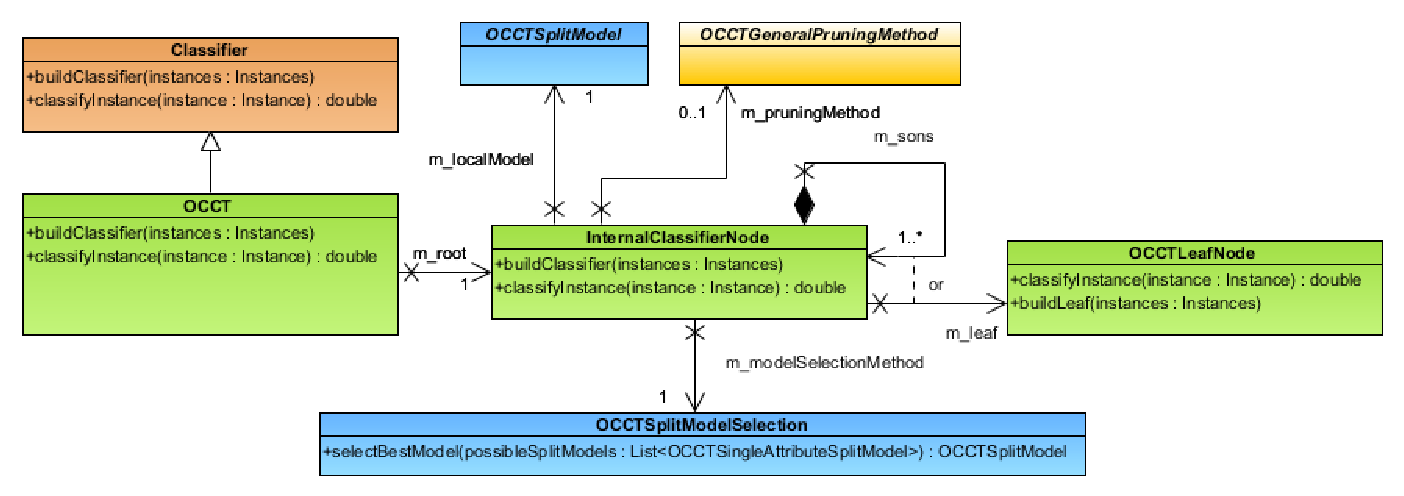
\includegraphics[width=1\textwidth]{Figures/ClassDiagrams/PDF/MainStructure.pdf}
    \caption{A UML Class diagram of the OCCT structure}
    \label{fig:main}
\end{figure}

\subsubsection{Splitting}\label{sec:splitting}
The split method can be of instance of one of the four proposed split criteria, e.g. represented by the {\em OCCTMaximumLikelihoodEstimationSplitModel class}. The base class for all the split methods is {\em OCCTSingleAttributeSplitModel}. This class contains methods for performing basic operations like calculating intersection and union between sets of instances which are required for some of the split criteria. All the split methods are instantiated using the Factory design pattern, so their creation logic is not exposed. The class {\em OCCTSplitModelFactory} serves as the Factory for creating all the  split methods. This is done by the {\em getSplitModel} static method. {\em OCCTSplitModelFactory} also serves for deciding about the best attribute to split by comparing the calculated scores for each attribute (e.g. implements the {\em chooseBestSplit} method, as explained  in~\cite{dror2011thesis,dror2014occt}). The UML Class Diagram which presents the structure of the classes which refer to splitting is presented in Figure~\ref{fig:splitting}.
\vspace{0.5cm}
\begin{figure}[!h]
    \centering
    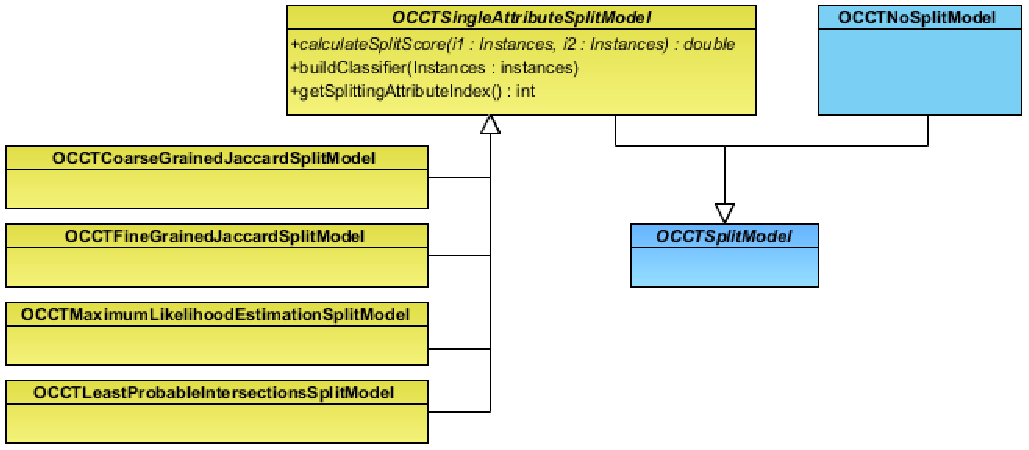
\includegraphics[width=1\textwidth]{Figures/ClassDiagrams/PDF/SplitMethods.pdf}
    \caption{A UML Class diagram of the OCCT Splitting criteria}
    \label{fig:splitting}
\end{figure}

\subsubsection{Leafs}
Each leaf of the tree is represented by the {\em OCCTLeafNodeClass} class and contains the built probabilistic models (which are represented by the {\em ProbModelsHandler} class). Also, as mentioned in \cite{dror2011thesis} and \cite{dror2014occt}, there is no need to save models for all possible attributes of $T_B$. Thus, a feature selection process is executed on the leaf dataset in order to choose the attributes that will be represented by the leafs. This is done by the {\em OCCTFeatureSelector} class which is instantiated for each internal node and extracts the attributes of leafs in case this node has leafs as children. The relevant UML Class Diagram is presented in Figure~\ref{fig:leafs}.
\vspace{0.5cm}
\begin{figure}[!h]
    \centering
    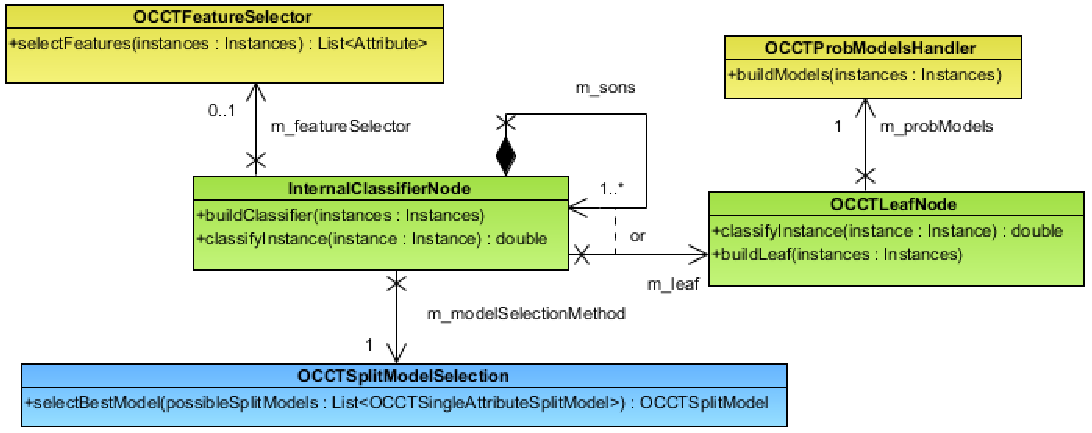
\includegraphics[width=1\textwidth]{Figures/ClassDiagrams/PDF/Leafs.pdf}
    \caption{A UML Class diagram of the classes which are relevant to leafs of OCCT}
    \label{fig:leafs}
\end{figure}

\subsubsection{Pruning}
The authors of OCCT chose to follow the prepruning approach and proposed two prepruning methods: based on Maximum-Likelihood Estimation (MLE) or on Least-Probable Intersections (LPI). We support the both methods in our code and allow the user to choose the pruning method to use, along with the option to not apply any pruning. Figure~\ref{fig:pruning} presents a UML Class Diagram which contains the classes relevant for implementation of pruning.
\vspace{0.5cm}
\begin{figure}[!h]
    \centering
    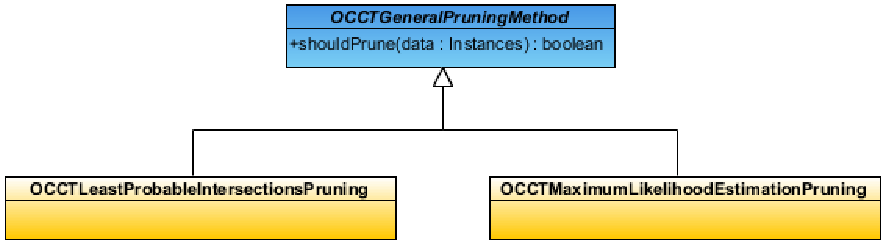
\includegraphics[width=1\textwidth]{Figures/ClassDiagrams/PDF/Pruning.pdf}
    \caption{A UML Class diagram of the classes which are relevant to pruning}
    \label{fig:pruning}
\end{figure}

\pagebreak

\subsection{Packages}
The packages structure of the code can be seen in Figure~\ref{fig:packages}. The designed structure allows an easy merge process with the existing Weka source code, as described in Section~\ref{sec:deployment}. The parent packages are {\em src.main.java.weka} which is similar to Weka directory structure presented in Figure~\ref{fig:wekadir}. Then, inside the {\em weka} package, there is {\em classifiers} package which contains different classifiers. Since our implementation was inspired from J48, only the main class, {\em OCCT.java} is located inside the main package {\em src.main.java.weka.trees.classifiers}, and all other parts of the implementation are located inside the internal {\em weka.classifiers.trees.occt} package.
\begin{figure}[!h]
\dirtree{%
.1 weka.
.2 classifiers.
.3 trees.
.4 occt.
.5 split.
.6 auxiliary.
.6 general.
.6 iterators.
.6 models.
.6 pruning.
.5 tree.
.5 utils.
.4 {\bf OCCT.java}.
}
    \caption{Packages structure of our OCCT implementation}
    \label{fig:packages}
\end{figure}

The internal {\em occt} package was divided to three packages: {\em split}, {\em tree} and {\em utils}. The first package, {\em occt.split}, contains all the parts of implementation which refer to the splitting methods, e.g. the {\em split.models} package contains implementation for the four split criteria proposed in~\cite{dror2011thesis,dror2014occt}. The {\em occt.tree} package contains the implementation of the tree structure for representing internal nodes and leafs of the tree, which are built during the training phase and queried during the testing phase. Finally, the {\em occt.utils} package contains some general auxiliary classes which are used in the
\pagebreak
%--------------------------------------------------------------------------------------------------------------------------------------------------
%	SECTION 4 - Deployment
%--------------------------------------------------------------------------------------------------------------------------------------------------
\section{Deployment}\label{sec:deployment}
In this Section we describe how to install and deploy our implementation of OCCT into a working source code of Weka. For simplicity we will describe the installation procedure under linux, installation for Windows is similar following the instructions below.

\subsection{Dependencies}
\subsubsection{Prerequisites}
First, please make sure you have GIT, Subversion and Ant installed.
if that is not the case, please use the following command:
\begin{lstlisting}[language=bash,frame=none,backgroundcolor=\color{anti-flashwhite}]
  $ sudo apt-get install git subversion ant
\end{lstlisting}

\subsubsection{Obtain Weka source code}
The OCCT code was implemented and evaluated on Weka stable version 3.6.12.
You will now have to checkout that specific branch by using the following svn checkout command:
\begin{lstlisting}[language=bash,frame=none,backgroundcolor=\color{anti-flashwhite}]
  $  svn co https://svn.cms.waikato.ac.nz/svn/weka/tags/stable-3-6-12 Weka-3-6-12
\end{lstlisting}
\newpar
A new directory named '{\em Weka-3-6-12}', will be created once the checkout procedure is done.
The directory structure will be as presented in Figure~\ref{fig:wekadir}.
\begin{figure}[!h]
\dirtree{%
.1 Weka-3-6-12.
.2 installer.
.3 \ldots{}.
.2 weka.
.3 build.
.3 lib.
.3 resources.
.3 src.
.4 main.
.5 java \begin{minipage}[t]{5cm} \textbf{$\textbf{<}$--- Please go here}\end{minipage}.
.6 weka.
.4 test.
.5 \ldots{}.
.2 wekadocs.
.3 \ldots{}.
.2 wekaexamples.
.3 \ldots{}.
}
    \caption{Weka directory structure}
    \label{fig:wekadir}
\end{figure}

\subsection{Installation}
The code structure of our OCCT implementation was carefully designed for fast deployment into the working source code of Weka. Before you fetch the latest build you first need get into the right path as shown in Figure~\ref{fig:wekadir}.
\begin{lstlisting}[language=bash,frame=none,backgroundcolor=\color{anti-flashwhite}]
  $ cd Weka-3-6-12/weka/src/main/java
\end{lstlisting}

\subsubsection{Synchronize with GIT}
Once in {\em Weka-3-6-12/weka/src/main/java} directory you will have to initialize the GIT repository in order to obtain the latest source files of our implementation.
Use the following commands to initialize and synchronize your local GIT repository with our latest build:
\begin{lstlisting}[language=bash,frame=none,backgroundcolor=\color{anti-flashwhite}]
  $ git init
  $ git remote add origin https://github.com/maortal/Weka.OCCT.Classifier.git
  $ git fetch
  $ git checkout -t origin/master
\end{lstlisting}
\newpar
On completion, a new directory named {\em occt} and an {\em OCCT.java} file will be added to your '{\em Weka-3-6-12/weka/src/main/java/weka/classifiers/trees}' directory.

\subsubsection{Compiling}
Now when the OCCT implementation is merged with Weka's source code, it is the time to compile the code. you need to travel back to '{\em Weka-3-6-12/weka}' directory and run {\em ANT} as follows:
\begin{lstlisting}[language=bash,frame=none,backgroundcolor=\color{anti-flashwhite}]
  $ cd ../../../
  $ ant exejar
\end{lstlisting}
Once compilation is complete, an executable jar file {\em weka.jar} is generated in a new folder named '{\em dist}'. This build of Weka contains our implementation of OCCT and can be ran using the standard java interface, e.g.:
\begin{lstlisting}[language=bash,frame=none,backgroundcolor=\color{anti-flashwhite}]
  $ cd dist
  $ java -jar weka.jar
\end{lstlisting}

%--------------------------------------------------------------------------------------------------------------------------------------------------
%	SECTION 5 - GUI Example
%--------------------------------------------------------------------------------------------------------------------------------------------------
\clearpage
\section{GUI Usage Example}
In this section we will show how to run OCCT, using the Explorer panel of Weka. We assume that the reader has some basic experience of working with Weka, but even an unexperienced user can run the algorithm by following the instructions below. In any case, the deployment stage (Section~\ref{sec:deployment}) should be performed in order to create an update {\em weka.jar} file which has the OCCT algorithm as one of the proposed classifiers.

\subsection{Preparing the Input}\label{sec:preparing_input}
The training and also the testing input data for the OCCT algorithm should be a single dataset $T_{AB}$ which contains only matching instances from $T_{A} \times T_{B}$. Each record, $r$, of the dataset is actually a pair of records $(r_{(a)},r_{(b)})$, one from the table $T_{A}$ and one from the table $T_{B}$, so that: $r=(r_{(a)},r_{(b)}) \in T_{AB} \subseteq T_{A} \times T_{B}$.

In the current version of the implementation, due to circumstances, we require all the attributes of $T_{A}$ to appear in the input dataset, followed by all the attributes of $T_{B}$. By this way, the attributes of $T_{B}$ can be pointed by a single index which refers to the first attribute of $T_{B}$ in the input dataset.

\begin{figure}[!h]
  \centering
  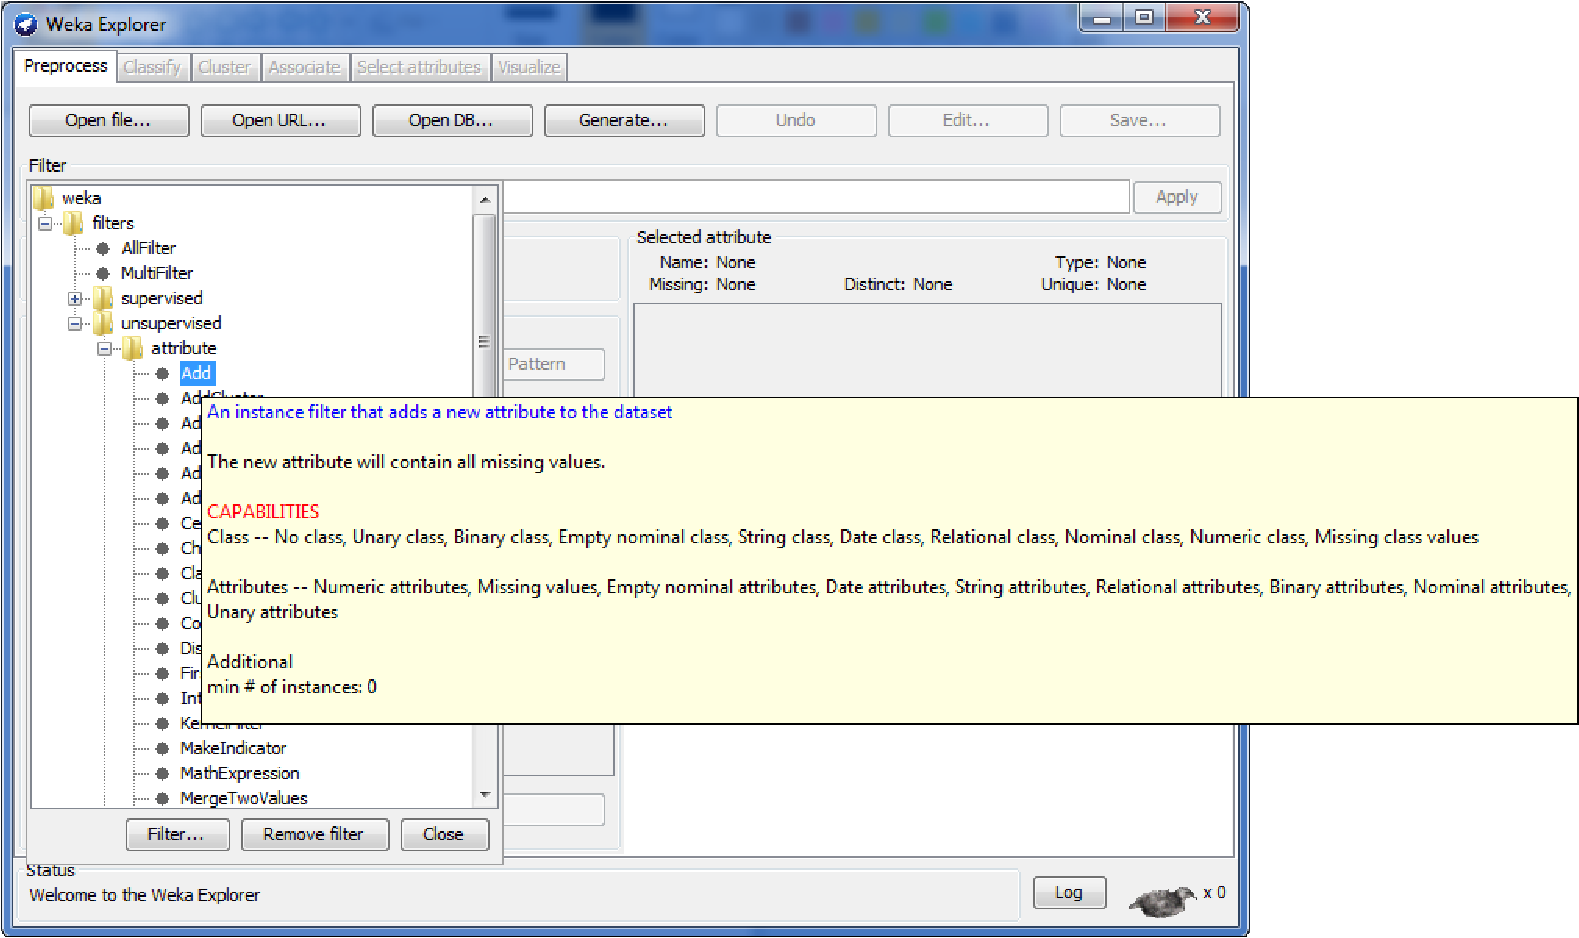
\includegraphics[width=1\textwidth]{Figures/GUI/PDF/AddFilter.pdf}
  \caption{Add filter, for adding the {\em 'IsMatch'} attribute}
  \label{fig:addfilter}
\end{figure}

We also require the input to contain a single attribute named {\em 'IsMatch'} which can receive two nominal values, {\em 'Match'} and {\em 'UnMatch'}, this attribute can be added to your input by using the unsupervised 'Add' attribute filter of Weka, from the 'Preprocess' tab (see Figure~\ref{fig:addfilter}).
Also note that the {\em IsMatch} attribute MUST be the last attribute of the dataset, i.e. located after the attributes of $T_{B}$. This attribute is required only for compatibility issues, thus, its values in the dataset are ignored and can be missing (of course they actually should be all {\em Match}). 
\subsection{Running the Algorithm}\label{sec:running}
In the Explorer panel (Figure~\ref{fig:wekaexplorer}), under {\em Preprocess} tab, click '{\em Open File...}' and select the preprocesses dataset, which is compatible with the requirements from the previous Section~(\ref{sec:preparing_input}). 
\begin{figure}[!t]
  \centering
  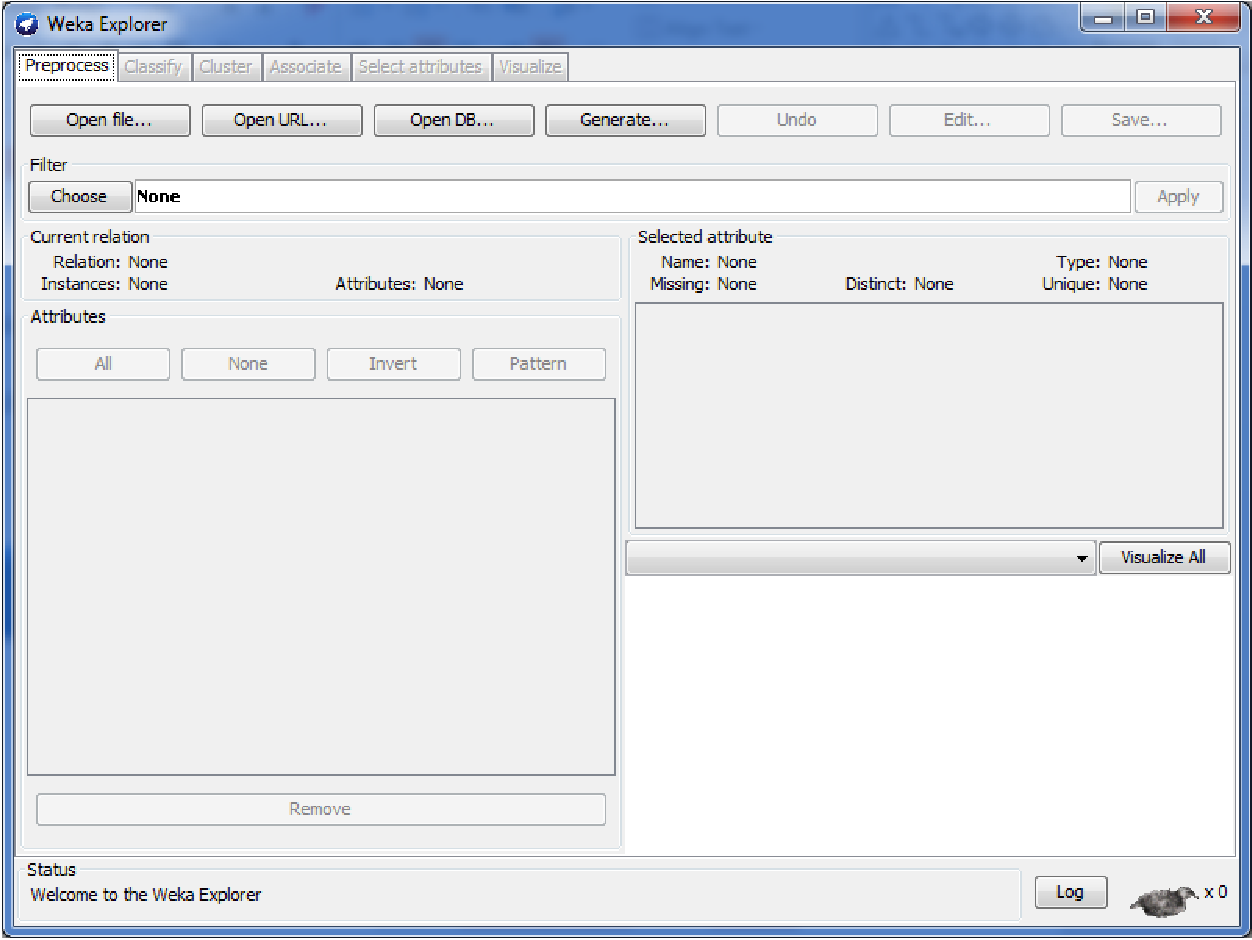
\includegraphics[width=0.8\textwidth]{Figures/GUI/PDF/MainExplorer.pdf}
  \caption{Explorer Panel of Weka}
  \label{fig:wekaexplorer}
\end{figure}
Under {\em Classify} tab, click on '{\em Choose}' and select {\em 'OCCT'} which is located under {\em tree} classifiers, as shown in Figure~\ref{fig:occtPre}. Now, you can configure the parameters of OCCT by clicking on the textbox which is located on the right side of the {\em 'Choose'} button. The available parameters are:

\begin{figure}[!t]
  \centering
  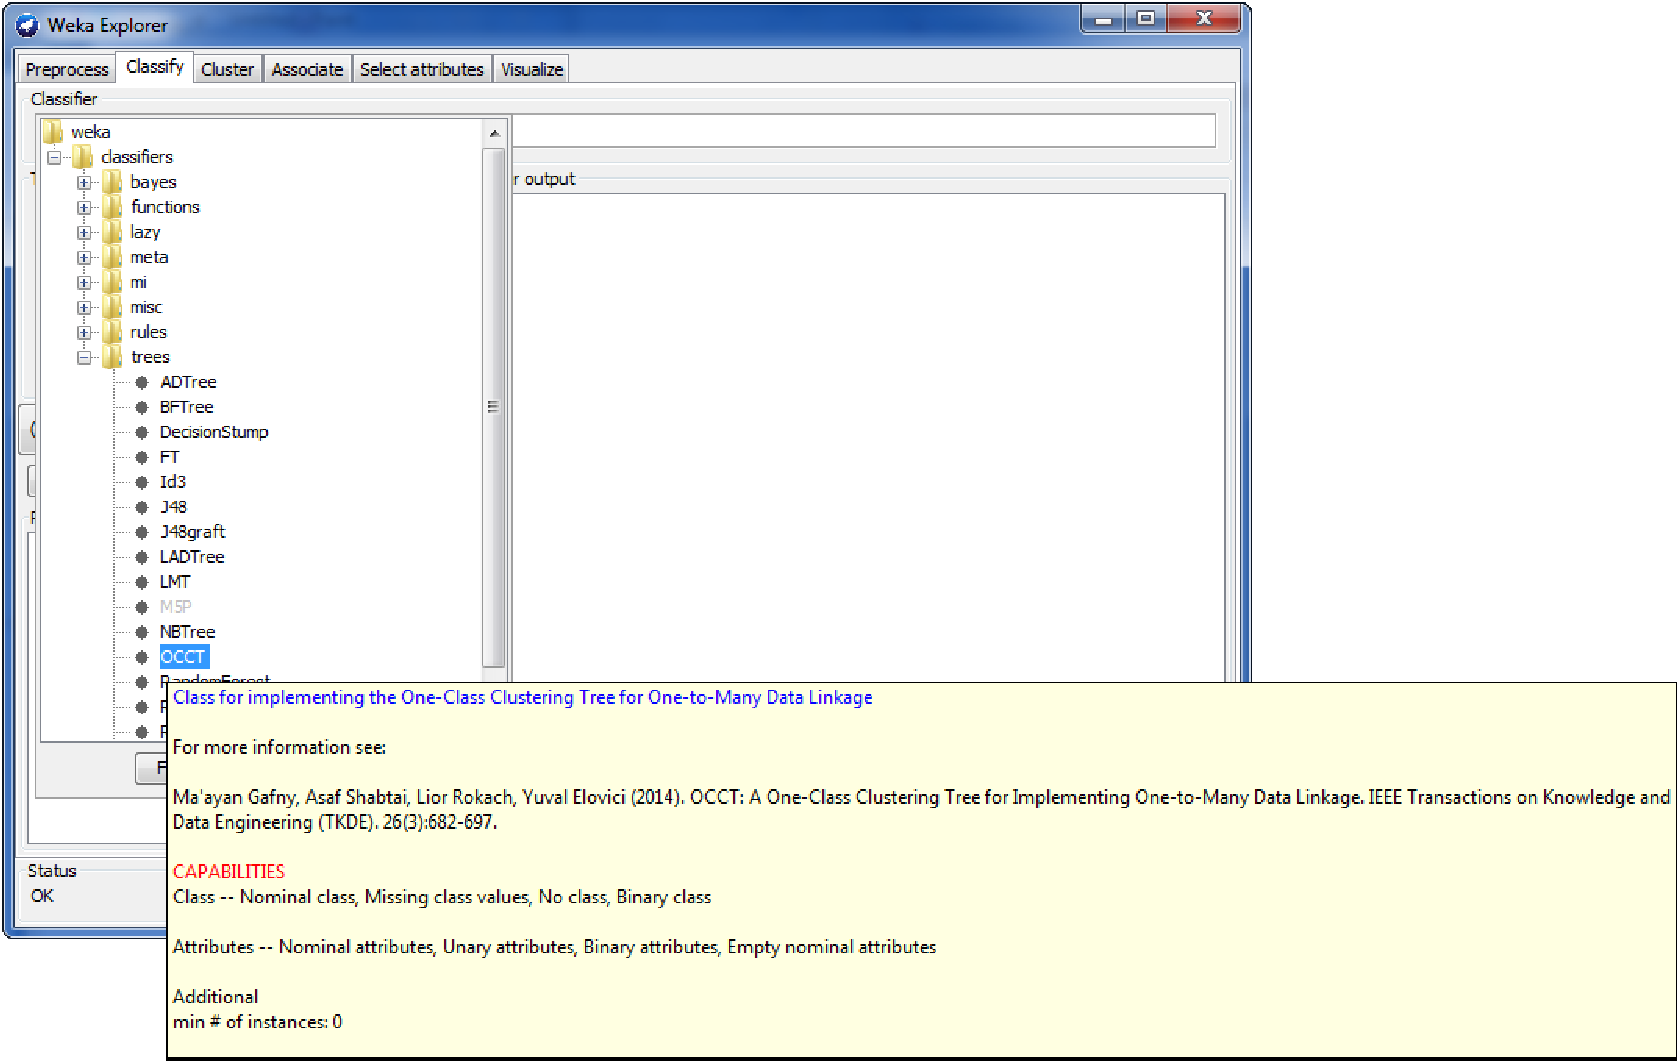
\includegraphics[width=1\textwidth]{Figures/GUI/PDF/OCCTPre.pdf}\vspace{1mm}
  \caption{The {\em Classify} tab of the Weka Explorer, with OCCT algorithm}
  \label{fig:occtPre}
\end{figure}

\begin{itemize}
  \item \textbf{{\em debug}} - A boolean flag which decides whether to print debugging information during the run.
  \item \textbf{{\em firstAttribueIndexOfB}} - since OCCT works on Cartesian product of two tables, you will need to provide it the index in where $T_{B}$ starts from. For further information refer to Section~\ref{sec:preparing_input}.
  \item \textbf{{\em linkageThreshold}} - During the testing phase, it is determined whether the given records are a match or not by comparing the likelihood score that was calculated, to the given threshold $th$. If the pair's score is greater than $th$, it is classified as a match otherwise, it is classified as a nonmatch. This parameter is used for defining $th$.
  \item \textbf{{\em pruningMethod}} - In order to reduce the time complexity of the algorithm, OCCT suggests two prepruning approaches.
  \begin{itemize}
    \item {\em Least-Probable Intersections (LPI)}
    \item {\em Maximum-Likelihood Estimation (MLE)}
  \end{itemize}
  By default, no pruning is performed.
  \item \textbf{{\em pruningThreshold}} - Sometimes, in order to determine whether to prune a branch or not. we need to compare its pruning method score with a given threshold. Currently, this threshold is used only in the {\em LPI} pruning method. In this method a score, $Z$ is calculated for each possible split and if for all possible splitting attributes this score is smaller than the predefined threshold, then we will not gain much information from any of the possible splits and the branch will be pruned.      
  \item \textbf{{\em splittingCriteria}} - In order to generate a tree with a small amount of nodes that generalize the data,
  it is crucial to use an effective splitting criterion. OCCT suggests four splitting methods:
  \begin{itemize}
    \item {\em Coarse-Grained Jaccard (CGJ)}
    \item {\em Fine-Grained Jaccard (FGJ)}
    \item {\em Least-Probable Intersections (LPI)}
    \item {\em Maximum-Likelihood Estimation (MLE)}
  \end{itemize}
  The default splitting criterion is {\em MLE}.
  \item \textbf{{\em useCardinality}} - A boolean flag, which determines whether to use cardinality in the data linkage state or not. By default, for simplification issues, cardinality is not used
\end{itemize}

\begin{figure}[!t]
  \centering
  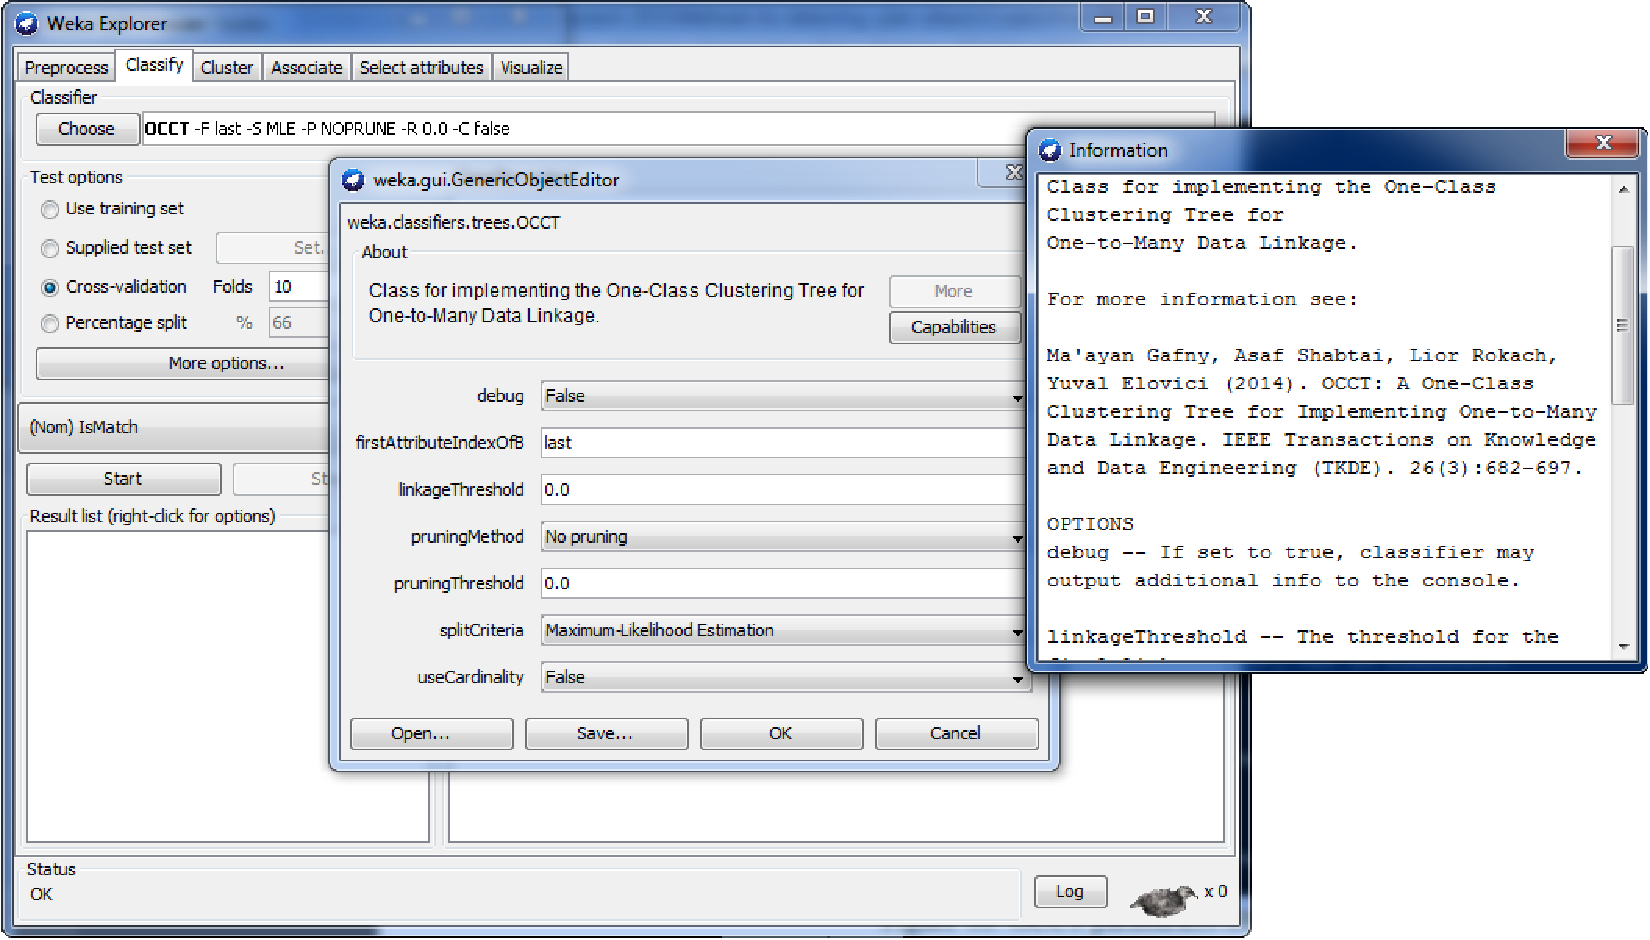
\includegraphics[width=1\textwidth]{Figures/GUI/PDF/OCCTConfig.pdf}
  \caption{OCCT parameters configuration window}
  \label{fig:occtconf}
\end{figure}

\subsection{Viewing the Results}
After configuring all the required parameters for OCCT, as described in the previous Section~(\ref{sec:running}), you can press the {\em 'Start'} button. The algorithm will perform training and possibly testing (accordingly to the requirement) and the created tree will be written to the {\em 'Classifier Output'} textbox, located at the right side of the window. See Figure~\ref{fig:occtview} for example.

\begin{figure}[!h]
  \centering
  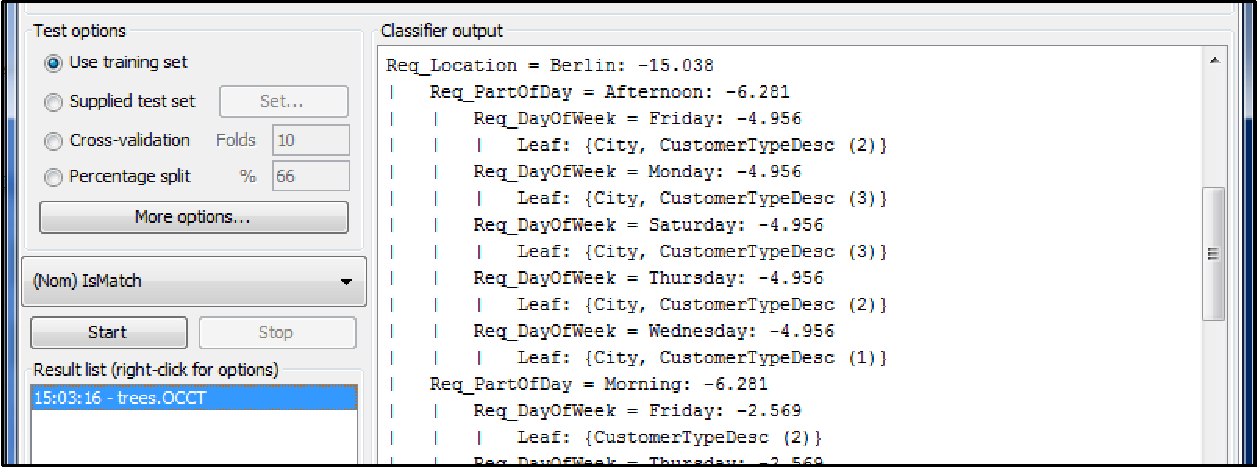
\includegraphics[width=0.9\textwidth]{Figures/GUI/PDF/OCCTViewTree.pdf}
  \caption{A decision tree induced by OCCT, presented in the Explorer window of Weka}
  \label{fig:occtview}
\end{figure}

%--------------------------------------------------------------------------------------------------------------------------------------------------
%	SECTION 6 - Code usage example
%--------------------------------------------------------------------------------------------------------------------------------------------------
\section{Code Usage Example}
Below you can seen an example of accessing the OCCT algorithm via Java code. In this example a dataset named {\em database\_misuse\_example\_with\_match.arff} is loaded (lines 3-6) and OCCT is applied on it, in order to induce a linkage model (lines 8-21). Once the model in created, it is tested against the first record of the dataset (lines 23-24).
\vspace{5mm}
\begin{lstlisting}
    public static void main(String [] argv) throws IOException {
        // load data from arff file
        BufferedReader reader = new BufferedReader(
            new FileReader(new File(argv[0], "database_misuse_example_with_match.arff")));
        Instances data = new Instances(reader);
        reader.close();
        // Train OCCT (don't add any fake class attribute).
        OCCT occt = new OCCT(true);
        // Set debugging mode ON.
        occt.setDebug(true);
        // Set splitting criteria to MLE.
        occt.setSplitCriteria(new SelectedTag(OCCT.SPLIT_MLE, OCCT.TAGS_SPLIT_CRITERIA));
        // Don't use pruning.
        occt.setPruningMethod(new SelectedTag(OCCT.PRUNING_NO_PRUNING, OCCT.TAGS_PRUNING_METHOD));
        // Make attributes of B be: "City", "CustomerTypeDesc" (1-based)
        occt.setFirstAttributeIndexOfB((data.attribute("City").index() + 1) + "");
        // Define the linkage threshold
        occt.setLinkageThreshold(1.0);
        // Run OCCT and print results
        try {
            occt.buildClassifier(data);
            System.out.println(occt.toString()); // System.out.println(occt.graph()); //print tree in dotfile format
            System.out.println("Classification: " +
                occt.classifyInstance(data.firstInstance()));
        } catch (Exception e) {
            e.printStackTrace();
        }
    }
\end{lstlisting}

%--------------------------------------------------------------------------------------------------------------------------------------------------
%	SECTION 7 - Evaluation
%--------------------------------------------------------------------------------------------------------------------------------------------------
\section{Evaluation}
We evaluated our implementation of OCCT using the same dataset that was used by the authors of OCCT (see Table~\ref{ref:datatable}). In this Section a side-by-side comparison of snapshots will be presented in-order to show that our implementation of OCCT algorithm is as intended by the authors.
\begin{table}[h]
\centering
\smaller
\begin{tabular}{|c|c|c|c|c|c|}\hline
  Request ID & Request Part Of Day & Request Day Of Week & Request Location & Customer City & Customer Type \\\hline
1          & Afternoon           & Friday              & Berlin           & Berlin        & private       \\\hline
2          & Afternoon           & Wednesday           & Hamburg          & Hamburg       & private       \\\hline
3          & Morning             & Wednesday           & Berlin           & Berlin        & business      \\\hline
4          & Morning             & Wednesday           & Berlin           & Berlin        & private       \\\hline
5          & Afternoon           & Saturday            & Berlin           & Berlin        & private       \\\hline
6          & Morning             & Thursday            & Berlin           & Berlin        & private       \\\hline
7          & Afternoon           & Friday              & Berlin           & Berlin        & private       \\\hline
8          & Afternoon           & Saturday            & Berlin           & Berlin        & business      \\\hline
9          & Afternoon           & Saturday            & Berlin           & Berlin        & private       \\\hline
10         & Afternoon           & Friday              & Hamburg          & Hamburg       & business      \\\hline
11         & Afternoon           & Monday              & Hamburg          & Hamburg       & business      \\\hline
12         & Afternoon           & Saturday            & Hamburg          & Hamburg       & private       \\\hline
13         & Afternoon           & Monday              & Berlin           & Berlin        & private       \\\hline
14         & Afternoon           & Monday              & Berlin           & Bonn          & private       \\\hline
15         & Afternoon           & Monday              & Berlin           & Berlin        & private       \\\hline
16         & Morning             & Saturday            & Bonn             & Bonn          & private       \\\hline
17         & Morning             & Saturday            & Hamburg          & Hamburg       & private       \\\hline
18         & Morning             & Saturday            & Hamburg          & Hamburg       & private       \\\hline
19         & Afternoon           & Friday              & Hamburg          & Hamburg       & private       \\\hline
20         & Afternoon           & Friday              & Hamburg          & Bonn          & private       \\\hline
21         & Morning             & Friday              & Hamburg          & Berlin        & private       \\\hline
22         & Morning             & Friday              & Berlin           & Berlin        & business      \\\hline
23         & Morning             & Friday              & Berlin           & Berlin        & private       \\\hline
24         & Afternoon           & Wednesday           & Berlin           & Berlin        & private       \\\hline
25         & Afternoon           & Thursday            & Berlin           & Berlin        & private       \\\hline
26         & Afternoon           & Thursday            & Berlin           & Berlin        & business      \\\hline
27         & Afternoon           & Monday              & Bonn             & Bonn          & business      \\\hline
28         & Afternoon           & Monday              & Bonn             & Hamburg       & private       \\\hline
29         & Afternoon           & Monday              & Bonn             & Berlin        & business      \\\hline
30         & Afternoon           & Wednesday           & Bonn             & Bonn          & business      \\\hline
31         & Afternoon           & Friday              & Bonn             & Bonn          & private       \\\hline
\end{tabular}
\caption{The training set that was used in our evaluation, same is in~\cite{dror2011thesis}}
\label{ref:datatable}
\end{table}


Pursuing the MLE splitting method with no pruning at al, in~\cite{dror2011thesis}, yielded the OCCT tree which is graphically presented in Figure~\ref{fig:originalMLEnoP}. Applying our implementation of OCCT on the same dataset and with the same parameters yielded the tree which is graphically presented in Figure~\ref{fig:ourMLEnoP}. As it can be seen, the two trees are similar.

Using the MLE pruning method on the same dataset and with the MLE splitting method, in~\cite{dror2011thesis}, yielded the OCCT tree which is graphically presented in Figure~\ref{fig:originalMLEwP}. Our implementation achieved the same tree when applying on the same dataset and setting the pruning method to be also MLE. The result tree we got, can be seen in Figure~\ref{fig:ourMLEwP}.
\pagebreak
\begin{figure}[!h]
    \centering
    \begin{subfigure}{\linewidth}        
        \vspace*{1cm}
        \centering
        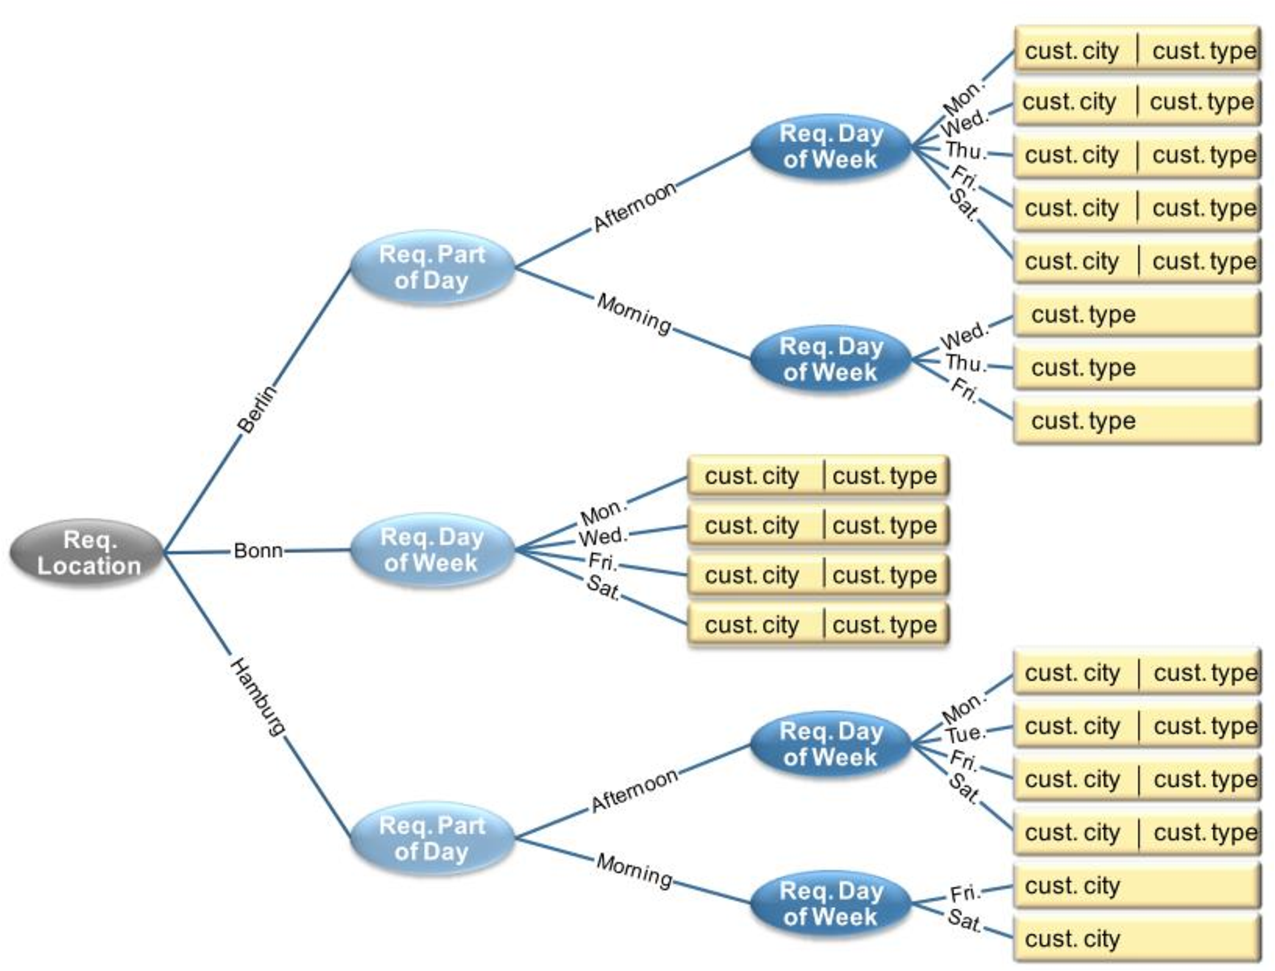
\includegraphics[width=1\textwidth]{Figures/Eval/PDF/MaayanMLEnoP.pdf}
        \caption{Decision model induced by Dror et al.~\cite{dror2011thesis} by using MLE with no pruning}\label{fig:originalMLEnoP}
        \vspace*{2cm}
    \end{subfigure}
    \begin{subfigure}{\linewidth}
        \centering
        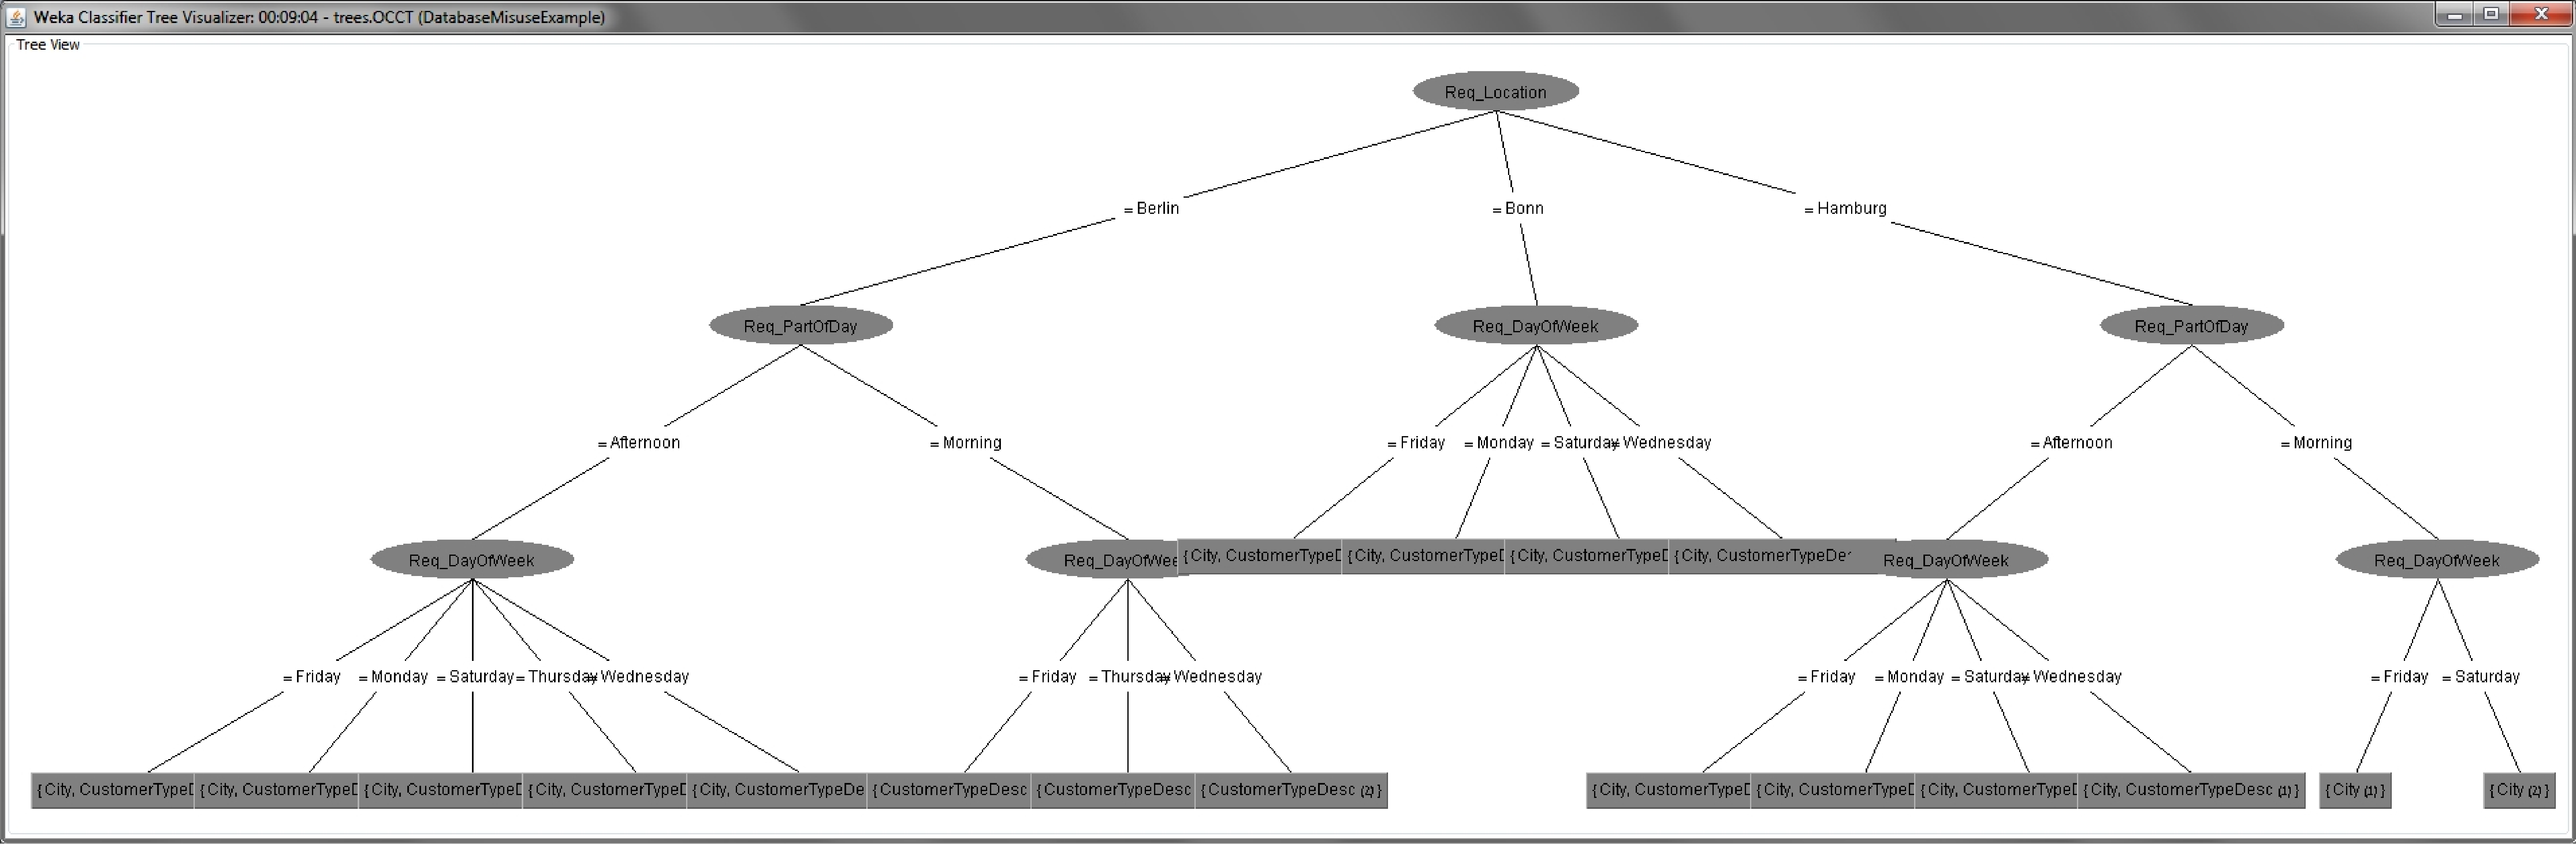
\includegraphics[width=1\textwidth]{Figures/Eval/PDF/OurMLEnoP.pdf}
        \caption{The tree induced by our implementation of OCCT, using MLE splitting criteria without pruning\\ (Snapshot taken from Weka tree visualizer)\\The induced model can be loaded from here \attachfile{Figures/Data/mle_no_pruning.model.txt}}\label{fig:ourMLEnoP}
    \end{subfigure}
\end{figure}
\pagebreak
\begin{figure*}[!h]
    \centering
    \begin{subfigure}{\linewidth}
        \vspace*{1cm}
        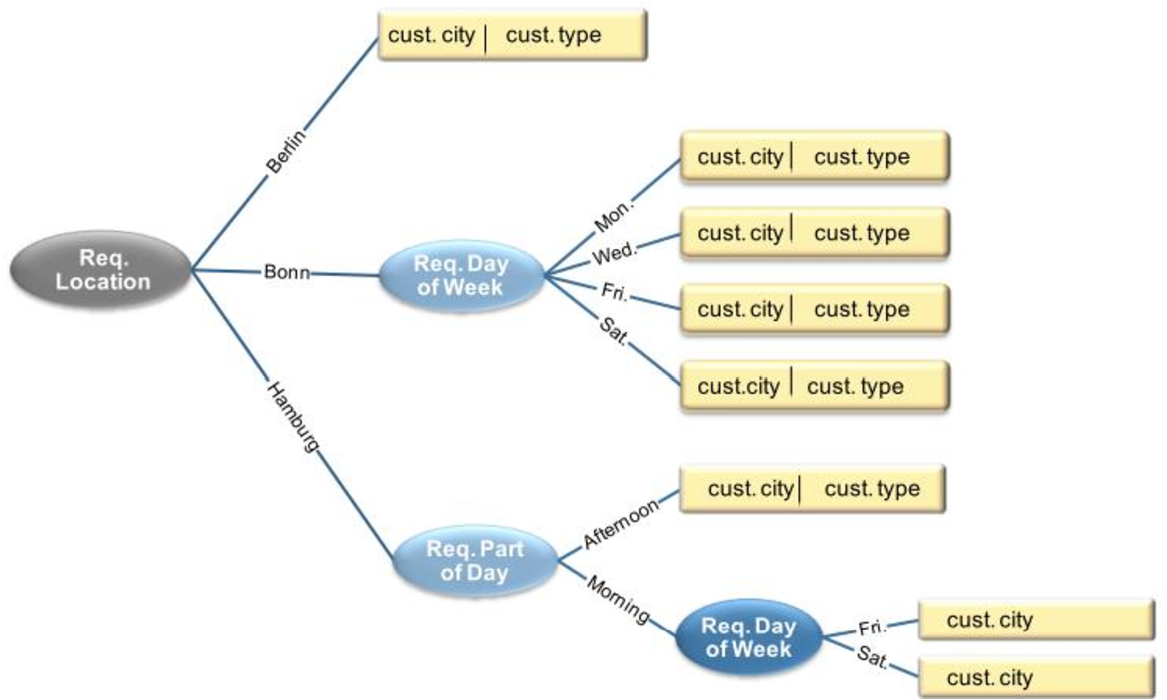
\includegraphics[width=1\textwidth]{Figures/Eval/PDF/MaayanMLEwP.pdf}
        \caption{Decision model induced by Dror et al.~\cite{dror2011thesis} by using MLE, with MLE pruning}\label{fig:originalMLEwP}
        \vspace*{3cm}
    \end{subfigure}
    \begin{subfigure}{1\textwidth}
        \centering        
        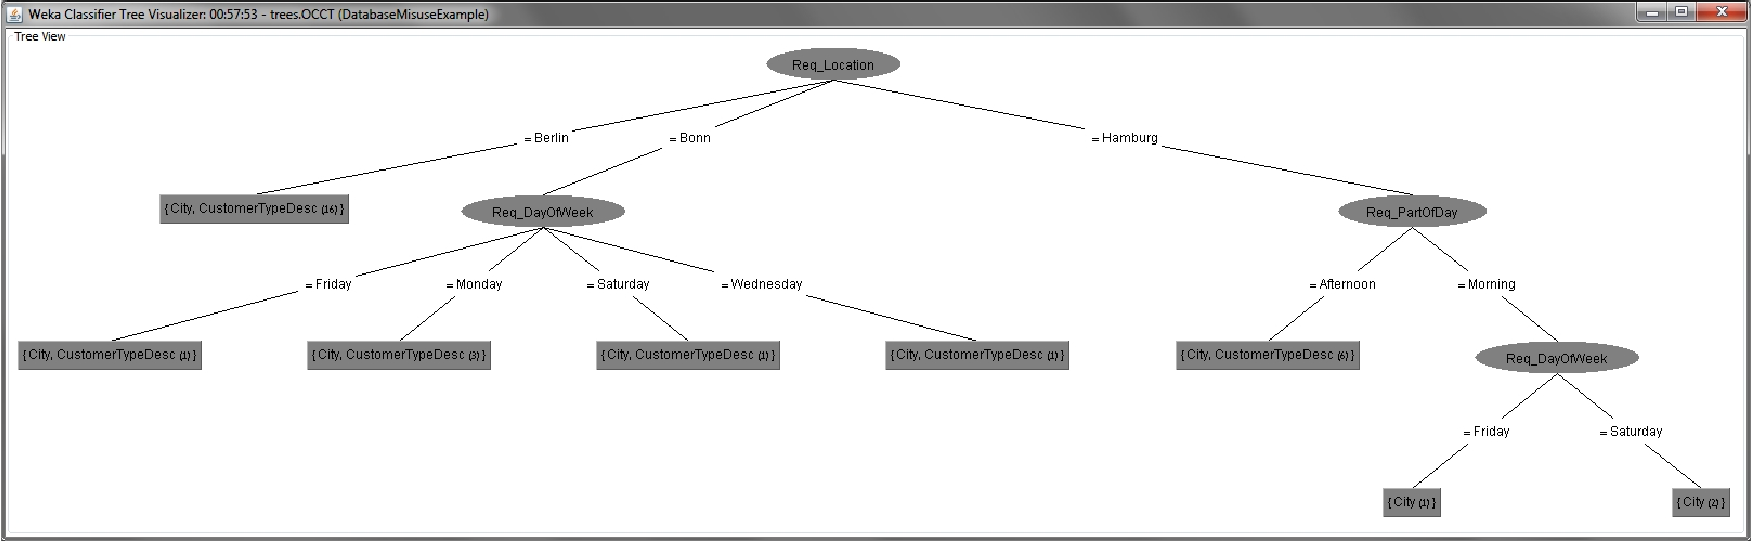
\includegraphics[width=1\textwidth]{Figures/Eval/PDF/OurMLEwP.pdf}
        \caption{The tree induced by our implementation of OCCT, using MLE splitting criteria, with MLE pruning\\ (Snapshot taken from Weka tree visualizer)\\The induced model can be loaded from here \attachfile{Figures/Data/mle_mle_pruning.model.txt}}\label{fig:ourMLEwP}
    \end{subfigure}
\end{figure*}
\pagebreak
%--------------------------------------------------------------------------------------------------------------------------------------------------
%	SECTION 8 - Future Work
%--------------------------------------------------------------------------------------------------------------------------------------------------
\section{Future Work and Extensions}
\begin{comment}
The major drawback of OCCT which has not been overcame in the implementation is too many possible configurations (four splitting criteria and two pruning methods). Thus, a characterization is required in order to decide which splitting criteria and pruning method should be used in each type of domain.
\end{comment}

There is still a lot of work that can be done in order to improve and extend the current implementation and allow it to be ran on more datasets.

First, as noted in \cite{dror2011thesis}, the proposed OCCT algorithm is only capable of handling discrete data. Thus, it cannot analyze attributes that consist of continuous values. In case either $T_A$ or $T_B$ has such attributes, some kind of discretization must be applied in order to make them semi-nominal. This discretization must be done during a preprocess step, before running OCCT. In the current version of the implementation, Weka disables the possibility to ran the algorithm on datasets if they have at least one attribute that is not nominal. This is implemented by using the {\em Capabilities} class of Weka, which ensures that features (e.g. handling certain types of attributes) are enabled explicitly. Our suggestion is to implement this missing functionality and allow OCCT to handle both continuous and discrete attributes. For example, handling continuous attributes can be implemented in the same way of C4.5, which creates a threshold and then splits the instances into those whose attribute value is above the threshold and those that are less than or equal to it.

Other problem with the current implementation refers to the input format of the algorithm; currently, OCCT is referred as a classification algorithm, which means that it is located under the {\em Classify} tab of Weka and uses the common GUI of a classifier. However, OCCT purpose is solving data linkage problems. The uniqueness of these problems is the input type which consists of two datasets. Also, the class attribute of the input dataset/s is irrelevant, since OCCT is a one-class data linkage algorithm. This type of input does not exist in the Classify tab of the GUI chooser of Weka. Currently, in order to overcome that problem of receiving two datasets as an input, we added an input index, which defines the first column of $T_B$ in the input (see Section~\ref{sec:preparing_input}). Since the input of the algorithm is a training set of only matching instances $T_{AB} \subseteq T_A \times T_B$, it is sufficient for now. However, Weka has an option of adding extra tabs in the Explorer in order to add new functionality without the hassle of having to dig into the code of the Explorer. We suggest to add a new tab for data linkage algorithms. This tab should be similar to the Classify tab, but it will allow the user to choose two different datasets for $T_A$ and $T_B$.


Finally, we propose to improve the efficiency of the implementation of the different split methods. This can be done by performing refactoring of the code. Also, we propose to use string matching algorithms which were suggested by Dror et. al.~\cite{dror2014occt}, in order to perform different tasks, e.g. finding an intersection between two subsets of records, in an efficient way.

%--------------------------------------------------------------------------------------------------------------------------------------------------
\bibliographystyle{unsrt}
\bibliography{refFile}
\restoregeometry
\end{spacing}

\end{document}
